% \section{}
\pagebreak
 \section*{Appendix 1 - Image Recognition \& Augmented Images}
 Image Recognition was also a really interesting feature to use, yet unfortunately it is not used in the application. This may have been able to be implemented, yet with the current implementations 
 of the landmark menu and the ARMode switching, It did not make much sense to be used. (As in the near landmark menu, there is no access to the camera), and the user may only use AR Mode when near a landmark.\\
 However, this feature is also fully working, and may easily be implemented if a better use in the context of outdoor AR is identified. 
 In the case of this project, a quick database manager was created in which a list of images could
  be inserted. These images also need to have specific features, to be distinguishable from other places (for example some image of plain grey gravel is not very easily distinguishable, 
  but an image of the earth is). And actions would be taken according to the image detected!
  \subsubsection*{Testing}
As augmented images were implemented some basic testing was also involved, where a simple image of the earth was detected, and overlayed with a 3D spinning globe. 
The image was recognized from different angles and light settings whilst tracking also was really responsive to even moving the image.
\begin{figure}[!htb]
    \minipage{0.32\textwidth}
        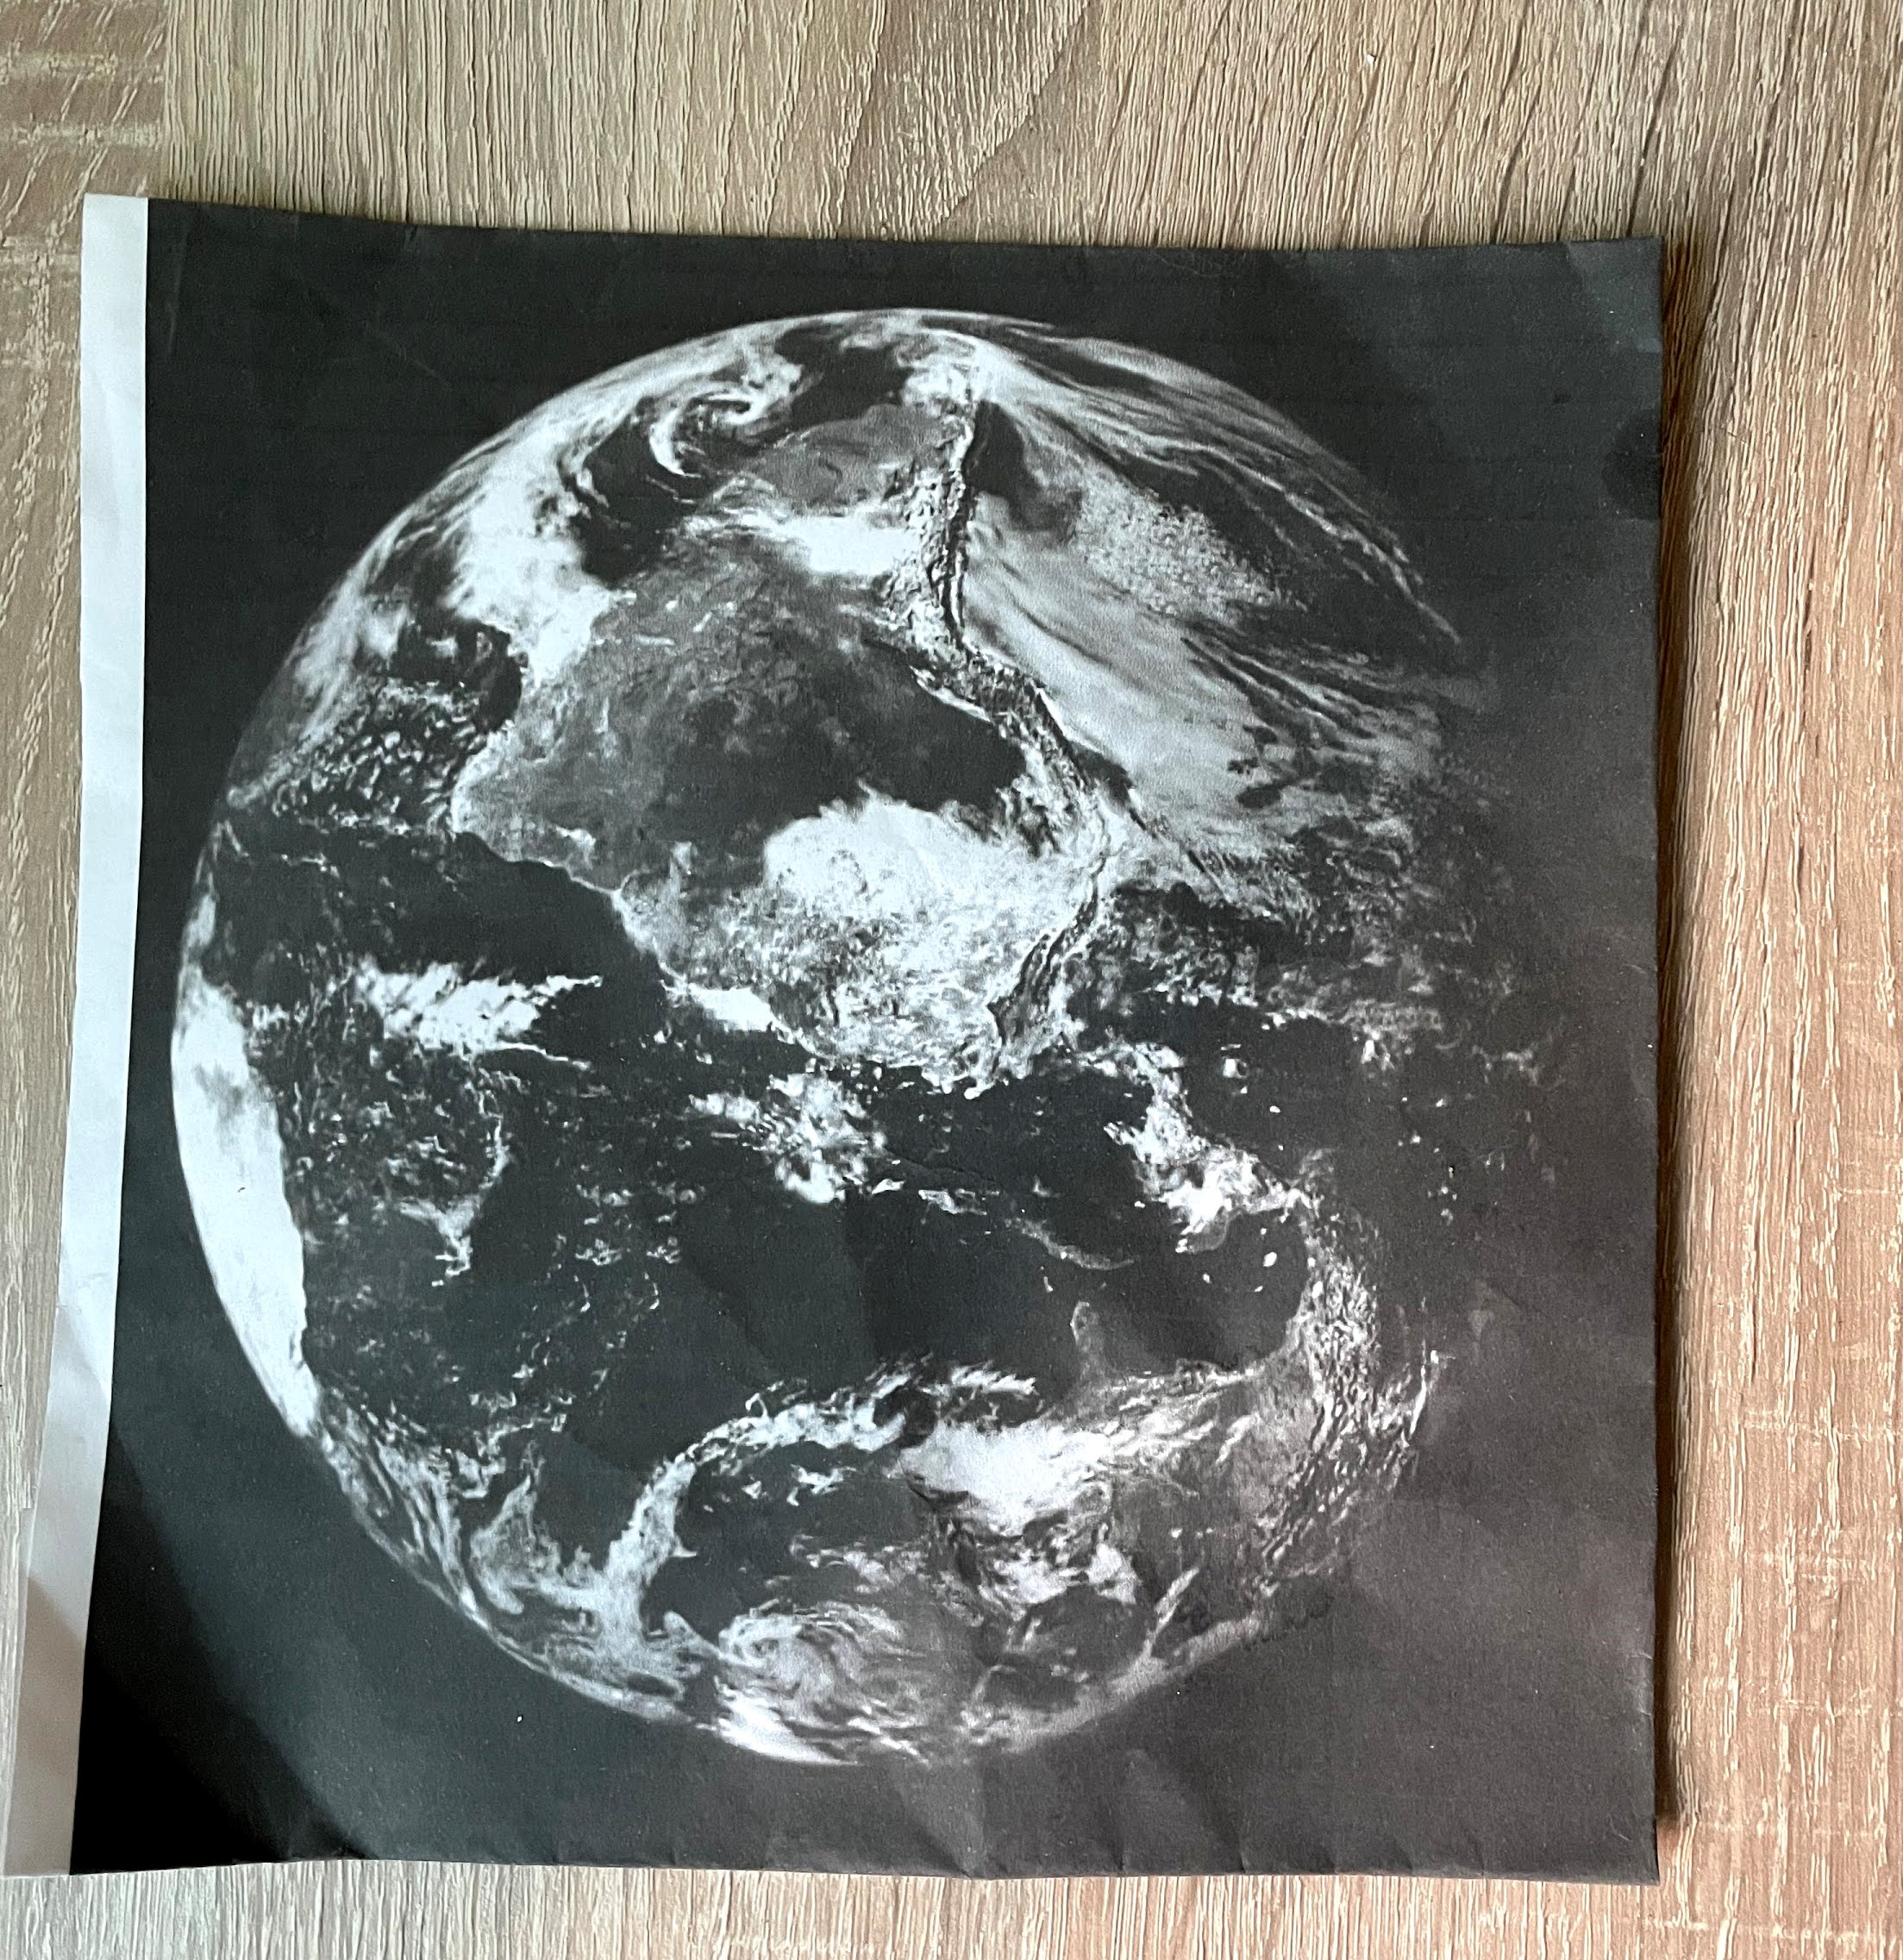
\includegraphics[width=\linewidth]{earth_og}
            \caption{Earth Image Key}
            \label{fig:earth_og}
    \endminipage\hfill
    \minipage{0.32\textwidth}
        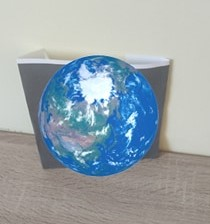
\includegraphics[width=\linewidth]{earth_ov}
        \caption{3D sphere overlayed}
        \label{fig:earth_ov}
    \endminipage
    \end{figure}